%%%%%%%%%%%%%%%%%%%%%%%%%%%%%%%%%%%%%%%%%%%%%%%%%%%%%%%%%%%%%%%%%%%%%%%%%%%%%%%%
% AMS Beamer series / Bologna FC / Template
% Andrea Omicini
% Alma Mater Studiorum - Università di Bologna
% mailto:andrea.omicini@unibo.it
%%%%%%%%%%%%%%%%%%%%%%%%%%%%%%%%%%%%%%%%%%%%%%%%%%%%%%%%%%%%%%%%%%%%%%%%%%%%%%%%
%\documentclass[handout]{beamer}\mode<handout>{\usetheme{default}}
%
\documentclass[presentation, 9pt]{beamer}\mode<presentation>{\usetheme{AMSBolognaFC}}
%\documentclass[handout]{beamer}\mode<handout>{\usetheme{AMSBolognaFC}}
%%%%%%%%%%%%%%%%%%%%%%%%%%%%%%%%%%%%%%%%%%%%%%%%%%%%%%%%%%%%%%%%%%%%%%%%%%%%%%%%
\usepackage[T1]{fontenc}
\usepackage{wasysym}
\usepackage{amsmath,blkarray}
\usepackage[minted,most]{tcolorbox}
\usepackage{centernot}
\usepackage{fontawesome}
\usepackage{fancyvrb}
\usepackage{minted}
\usepackage{hyperref}
\usepackage{multicol}
\setminted[scala]{fontsize=\scriptsize,baselinestretch=1,obeytabs=true, tabsize=2}
\usepackage[ddmmyyyy]{datetime}
\setminted{fontsize=\footnotesize}
\renewcommand{\dateseparator}{}
%\renewcommand{\thefootnote}{\fnsymbol{footnote}}
\newcommand{\version}{1}
\usepackage[
	backend=biber,
	citestyle=authoryear-icomp,
	maxcitenames=1,
	bibstyle=numeric]{biblatex}

	\makeatletter

\addbibresource{biblio.bib}
%%%%%%%%%%%%%%%%%%%%%%%%%%%%%%%%%%%%%%%%%%%%%%%%%%%%%%%%%%%%%%%%%%%%%%%%%%%%%%%%
\title[Reinforcement Learning]
{Reinforcement Learning}
\subtitle{An introduction}
%
%
\author[\sspeaker{Aguzzi}]
{\speaker{Gianluca Aguzzi} \href{mailto:gianluca.aguzzi@unibo.it}{gianluca.aguzzi@unibo.it}}
%
\institute[DISI, Univ.\ Bologna]
{Dipartimento di Informatica -- Scienza e Ingegneria (DISI)\\
\textsc{Alma Mater Studiorum} -- Universit{\`a} di Bologna \\[0.5cm]
\textbf{Talk @} \bold{Advanced School in Artificial Intelligence (ASAI)}}
%
\renewcommand{\dateseparator}{/}
\date[\today]{\today}
%
\AtBeginSection[]
{
  \begin{frame}
  \frametitle{Contents}
  \tableofcontents[currentsubsection, 
	sectionstyle=show/shaded, 
	subsectionstyle=show/shaded]
  \end{frame}
}
\AtBeginSubsection[]
{
  \begin{frame}
  \frametitle{Contents}
  \tableofcontents[currentsubsection, 
	sectionstyle=show/shaded, 
	subsectionstyle=show/shaded]
  \end{frame}
}
%%%%%%%%%%%%%%%%%%%%%%%%%%%%%%%%%%%%%%%%%%%%%%%%%%%%%%%%%%%%%%%%%%%%%%%%%%%%%%%%
\begin{document}
%%%%%%%%%%%%%%%%%%%%%%%%%%%%%%%%%%%%%%%%%%%%%%%%%%%%%%%%%%%%%%%%%%%%%%%%%%%%%%%%

%/////////
\frame{\titlepage}
%/////////
\begin{frame}{Hello World!}
	\begin{columns}
		\begin{column}{0.5\textwidth}
		\centering
		\fbox{
\includegraphics[width=0.5\linewidth]{img/me.jpeg}}
		\\
		\vspace{0.2cm}
		\href{https://github.com/cric96}{\faGithub} \,
		\href{https://stackoverflow.com/users/10295847/gianluca-aguzzi}{\faStackOverflow} \,
		\href{https://www.linkedin.com/in/gianluca-aguzzi-265998170/}{\faLinkedin} \,
		\href{https://www.unibo.it/sitoweb/gianluca.aguzzi}{\faGlobe} \,
		\end{column}
		\begin{column}{0.5\textwidth}
			\begin{itemize}
				\item PhD student in Computer Science and Engineering
				\item Research interests:
				\begin{itemize}
					\item Multi-agent systems
					\item Distributed Collective Intellingence
					\item Deep Reinforcement Learning
					\item Multi-agent Reinforcement Learning
					\item Distributed Macro-programming
				\end{itemize}
				%\item Lead developer of \href{https://scafi.github.io/}{ScaFi}
				%\item Scala Lover \& Functional Programming enthusiast
			\end{itemize}
		\end{column}
	\end{columns}
\end{frame}
\begin{frame}{Resources}
\begin{itemize}
	\item \emph{An Introduction to Reinforcement Learning}, Sutton and Barto,1998
	\begin{itemize}
		\item Available online at \url{http://incompleteideas.net/book/the-book-2nd.html}
	\end{itemize}
	\item \emph{Foundations of Deep Reinforcement Learning: Theory and Practice in Python}, Laura Graesser and Wah Loon Keng, 2020
	\item \emph{Deep Mind Lectures}:
	\begin{itemize}
		\item \textbf{Introduction to Reinforcement Learning with David Silver}: \url{https://www.deepmind.com/learning-resources/introduction-to-reinforcement-learning-with-david-silver}
		\item \textbf{Reinforcement Learning Lecture Series}: \url{https://www.deepmind.com/learning-resources/reinforcement-learning-lecture-series-2021}
	\end{itemize}
\end{itemize}
\end{frame}
%===============================================================================
\section{Introduction}
%===============================================================================
\begin{frame}[plain,c]
	%\frametitle{A first slide}
	\begin{center}
	\Huge What is Reinforcement Learning?
	\end{center}
\end{frame}

\begin{frame}[plain,c]
	%\frametitle{A first slide}
	\begin{center}
	\Huge What is Intelligence?
	\\
	\huge \emph{To able to \textbf{learn} to make \textbf{decisions} to achive \textbf{goals}}
	\end{center}
\end{frame}
\begin{frame}{What is Reinforcement Learning?}
\begin{itemize}
	\item Animals learn by interacting with our environment
	\begin{itemize}
		\item Babies learn how to communicate by interacting with parents
		\item Dogs learn how to behave by following the owner's orders
		\item Me learn how to surfing by falling from the surfboard
	\end{itemize}
	\item Difference from supervised learning:
	\begin{itemize}
		\item \textbf{active} learning (learn by doing)
		\item \textbf{sequential} interaction 
	\end{itemize}
	\item Learning guided by \textbf{goal} (goal-directed)
	\item Learning without examples \faArrowRight \, guided by reward signal
\end{itemize}
\end{frame}

\begin{frame}{Interaction loop}
\centering
\Large An \textbf{agent} interacts with the \textbf{environment} by perceive an \textbf{observation} and take an \textbf{action} accordingly which leads to a \textbf{reward}
\\
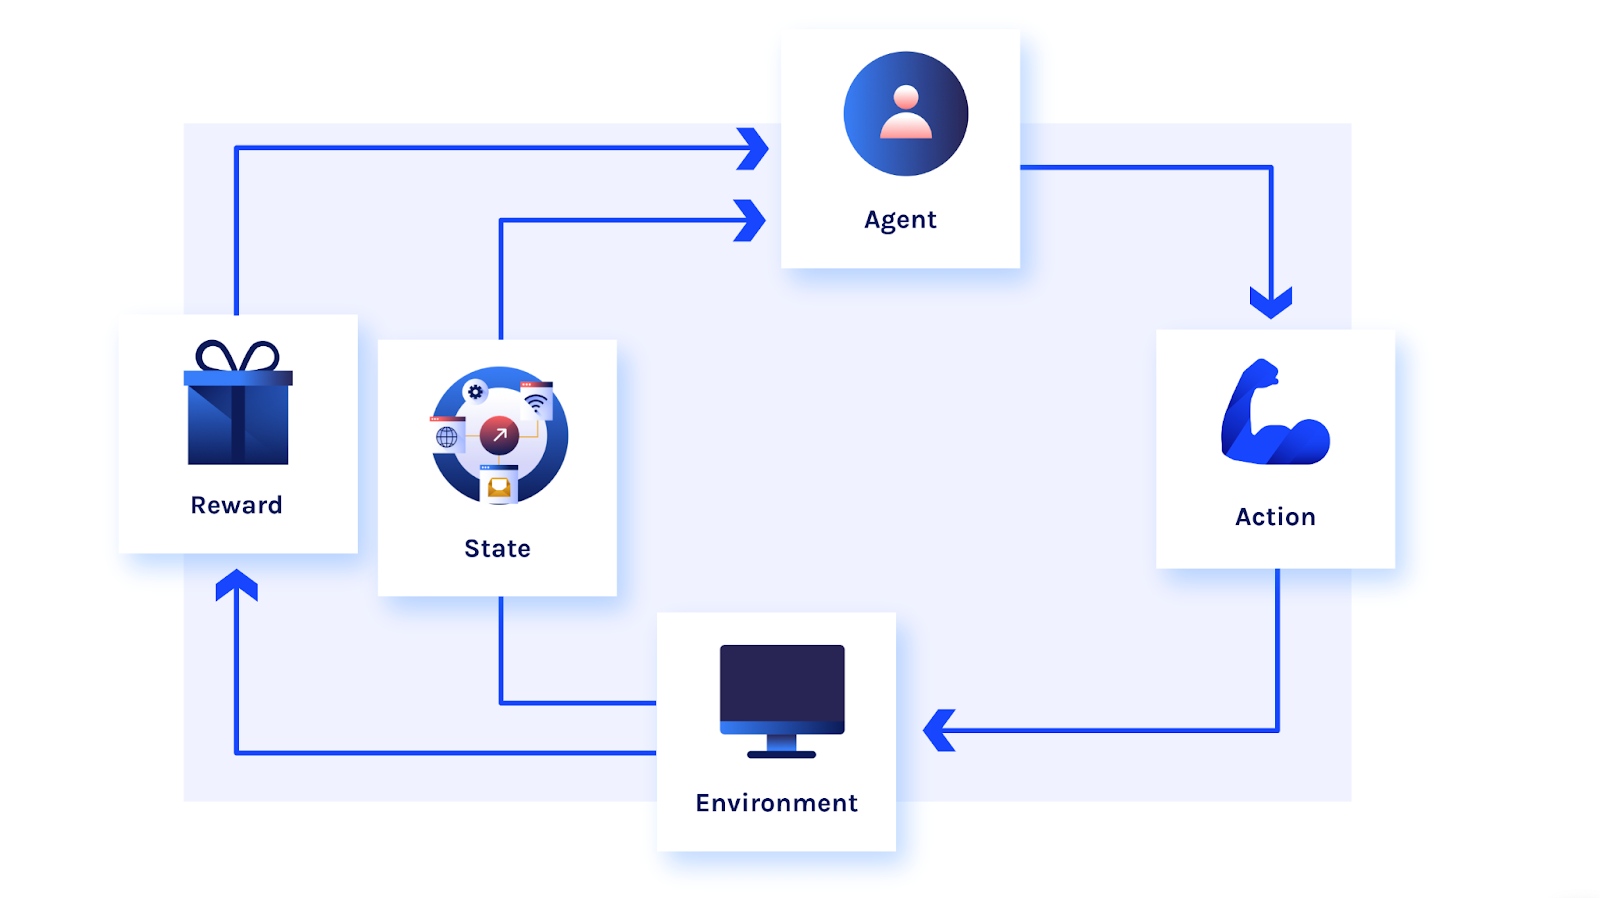
\includegraphics[height=6cm]{img/interaction-loop.png}
\\
\Large
\bold{Goal}: maximize the \textbf{cumulative reward} over time
\end{frame}

\begin{frame}{On problem expressiveness: reward hypothesis}
\begin{block}{Reward hypothesis}
\emph{Any goal can be formalized as the outcome of maximizing a cumulative reward}
\begin{itemize}
	\item Reinforcement learning is based on this hypothesis
	\item Ideally, we can formalize any problem as a reinforcement learning problem
\end{itemize}
\end{block}

\begin{alertblock}{Stronger statement: reward is enough}
\emph{intelligence, and its associated abilities, can be understood as subserving the maximisation of reward by an agent acting in its environment.}
\begin{itemize}
	\item Really controversial
\end{itemize}
\end{alertblock}
\end{frame}

\begin{frame}{Examples of Reinforcement Learning problems}
\begin{multicols}{2}
	\begin{itemize}
		\item Learning how to surf
		\item Managing a portfolio of cryptocurrencies
		\item Controlling the battery of an electric car 
		\item Playing chessboard
		\item Solving a cubic cube
	\end{itemize}
	\begin{itemize}
		\item[\faArrowRight] \textbf{Reward:} surfing time on the wave
		\item[\faArrowRight] \textbf{Reward:} money earned
		\item[\faArrowRight] \textbf{Reward:} battery level at the end of the day
		\item[\faArrowRight] \textbf{Reward:} win the game
		\item[\faArrowRight] \textbf{Reward:} solving time 
	\end{itemize}
\end{multicols}
\large
\textbf{NB!} if the goal is learn via environment interaction, then these are all reinforcement learning problems, regardless the algorithm involved
\end{frame}

\begin{frame}{Again, What is Reinforcement Learning}
\begin{itemize}
	\item There are several reasons why we should learn:
	\begin{enumerate}
		\item Find \textbf{solutions}
		\begin{itemize}
			\item A robot that reaches a target
			\item A program that plays chess (really well)
		\end{itemize}
		\item Adapt \textbf{online} (dealing with unknowns)
		\begin{itemize}
			\item A robot that learns how to walk in a new environment
			\item A program that learns how to play a new game
		\end{itemize}
	\end{enumerate}
	\item Reinforcement learning is used in both cases
	\item Adapting online is more challenging, and it is not just generalization (e.g. supervised learning)
\end{itemize}

\end{frame}

\begin{frame}{Motivating real world examples}
\centering
\href{https://www.youtube.com/watch?v=V1eYniJ0Rnk}{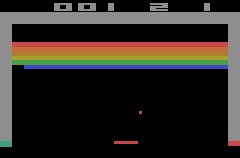
\includegraphics[width=0.32\textwidth]{img/atari.png}}
\href{https://www.youtube.com/watch?v=43cO39XBPIA}{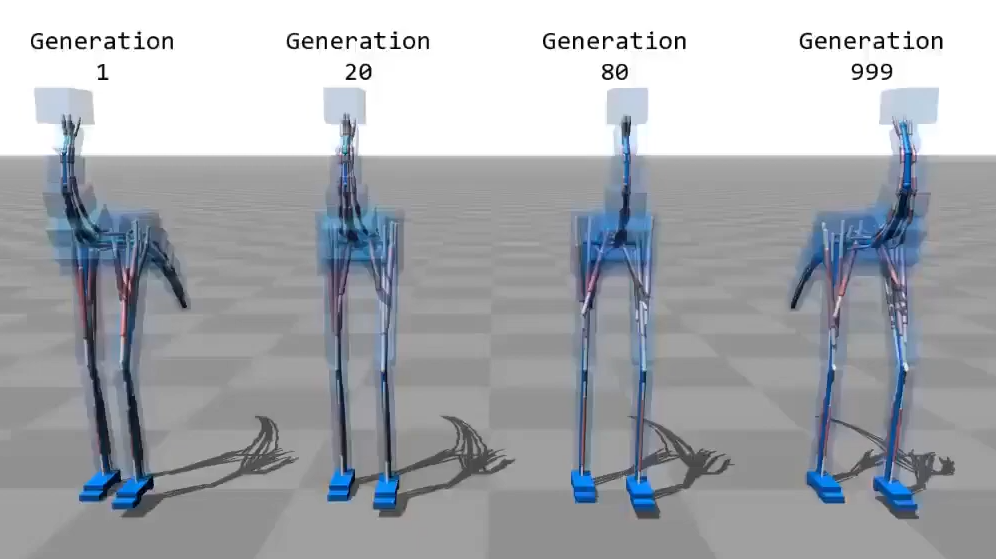
\includegraphics[width=0.32\textwidth]{img/robots.png}}
\href{https://www.youtube.com/watch?v=gn4nRCC9TwQ}{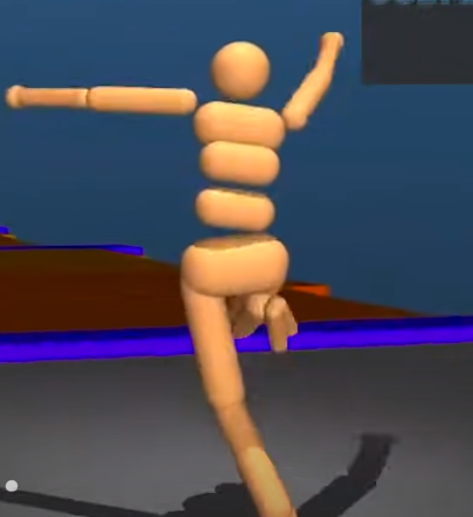
\includegraphics[width=0.32\textwidth]{img/ppo.png}}
\end{frame}
%===============================================================================
\section*{}
%===============================================================================

%/////////
\frame{\titlepage}
%/////////

%===============================================================================
\section*{\refname}
%===============================================================================

%%%%
\setbeamertemplate{page number in head/foot}{}
%/////////
\begin{frame}[c,noframenumbering, allowframebreaks]{\refname}
%\begin{frame}[t,allowframebreaks,noframenumbering]{\refname}
	\tiny
	\nocite{*}
	\printbibliography
\end{frame}
%/////////

%%%%%%%%%%%%%%%%%%%%%%%%%%%%%%%%%%%%%%%%%%%%%%%%%%%%%%%%%%%%%%%%%%%%%%%%%%%%%%%%
\end{document}
%%%%%%%%%%%%%%%%%%%%%%%%%%%%%%%%%%%%%%%%%%%%%%%%%%%%%%%%%%%%%%%%%%%%%%%%%%%%%%%%
